\documentclass[
	12pt,				% tamanho da fonte
	oneside,			% para impressão em verso e anverso. Oposto a oneside
	a4paper,			% tamanho do papel. 
	brazil				% o último idioma é o principal do documento]{article}
]{abntex2}

% ---
% Pacotes básicos 
% ---
%\usepackage{fontspec}

\usepackage[utf8]{inputenc}		% Codificacao do documento (conversão automática dos acentos)
\usepackage[T1]{fontenc}
\usepackage{indentfirst}		% Indenta o primeiro parágrafo de cada seção.
\usepackage{color}				% Controle das cores
\usepackage{graphicx}			% Inclusão de gráficos
\usepackage{microtype} 			% para melhorias de justificação
\usepackage{multicol}			% multiplas colunas no texto
% ---

% ---
% Pacotes de citações
% ---
\usepackage[brazilian]{backref}	 % Paginas com as citações na bibl
\usepackage[alf]{abntex2cite}	% Citações padrão ABNT


\usepackage{hyperref} % criar hyperlinks
\usepackage{listings} % utilizado para dar highlight em código
\usepackage[dvipsnames]{xcolor}
\usepackage[export]{adjustbox}

% --- 
\usepackage{hyperref} % criar hyperlinks
\usepackage{listings} % utilizado para dar highlight em código
\usepackage[dvipsnames]{xcolor}
\usepackage[export]{adjustbox}
\usepackage[top=3cm, bottom=2cm, left=3cm, right=2cm]{geometry}
\renewcommand{\baselinestretch}{1.5} % espaçamento entre linhas
%\setlength{\parskip}{0.5cm} % espaçamento entre paragrafos
%\setlength{\parindent}{2cm} % recuo do parágrafo
\usepackage{times}
% ---


\lstdefinestyle{customc}{ %custom color para código do arduino
  belowcaptionskip=1\baselineskip,
  backgroundcolor=\color{lightgray},
  breaklines=true,
  frame=single,
  xleftmargin=\parindent,
  language=C,
  showstringspaces=false,
  basicstyle=\footnotesize\ttfamily,
  keywordstyle=\bfseries\color{ForestGreen},
  commentstyle=\itshape\color{darkgray},
  identifierstyle=\color{blue},
  stringstyle=\color{gray},
  breaklines=true,
  morekeywords={bool},
}

% --- 
% CONFIGURAÇÕES DE PACOTES
% --- 

% ---
% Configurações do pacote backref
% Usado sem a opção hyperpageref de backref
\renewcommand{\backrefpagesname}{Citado na(s) página(s):~}
% Texto padrão antes do número das páginas
\renewcommand{\backref}{}
% Define os textos da citação
\renewcommand*{\backrefalt}[4]{
	\ifcase #1 %
		Nenhuma citação no texto.%
	\or
		Citado na página #2.%
	\else
		Citado #1 vezes nas páginas #2.%
	\fi}%
% ---

% ---
% Informações de dados para CAPA e FOLHA DE ROSTO
% ---
\titulo{Sistema de acompanhamento de transporte público para deficientes visuais }
\autor{Arthur Cicuto Pires\\Victor Vieira Paulino}
\local{Santo André}
\data{2017}


\instituicao{%
  Centro Universitário Fundação Santo André -- CUFSA
  \par
  Engenharia de Computação com Ênfase em Software}
  
\tipotrabalho{Conclusão de Curso}
% O preambulo deve conter o tipo do trabalho, o objetivo, 
% o nome da instituição e a área de concentração 
\orientador{Prof. Dr. Marcos Forte}
\preambulo{Trabalho de Conclusão de Curso apresentado à Faculdade de Engenharia “Engenheiro Celso Daniel” do Centro Universitário Fundação Santo André, como exigência parcial para obtenção do grau de Bacharel em Engenharia de Computação.}
% ---

% ---
% Configurações de aparência do PDF final

% alterando o aspecto da cor azul
\definecolor{blue}{RGB}{41,5,195}

% informações do PDF
\makeatletter
\hypersetup{
     	%pagebackref=true,
		pdftitle={\@title}, 
		pdfauthor={\@author},
    	pdfsubject={\imprimirpreambulo},
	    pdfcreator={LaTeX with abnTeX2},
		colorlinks=true,       		% false: boxed links; true: colored links
    	linkcolor=blue,          	% color of internal links
    	citecolor=blue,        		% color of links to bibliography
    	filecolor=magenta,      		% color of file links
		urlcolor=blue,
		bookmarksdepth=4
}
\makeatother
% --- 

% --- 
% Espaçamentos entre linhas e parágrafos 
% --- 

% O tamanho do parágrafo é dado por:
\setlength{\parindent}{1.3cm}

% Controle do espaçamento entre um parágrafo e outro:
\setlength{\parskip}{0.2cm}  % tente também \onelineskip

% ---
% compila o indice
% ---
\makeindex
% ---

% ----
% Início do documento
% ----

\begin{document}

% Seleciona o idioma do documento (conforme pacotes do babel)
%\selectlanguage{english}
%\selectlanguage{brazil}

% Retira espaço extra obsoleto entre as frases.
\frenchspacing 

% ----------------------------------------------------------
% ELEMENTOS PRÉ-TEXTUAIS
% ----------------------------------------------------------
% \pretextual
\begin{figure}[h]
\centering % este comando é usado para centralizar a figura

\includegraphics[width=4.5cm, height=2cm]{images/logo-fsa.jpg}\\
\end{figure}
% ---
% Capa
% ---
\imprimircapa
% ---

% ---
% Folha de rosto
% (o * indica que haverá a ficha bibliográfica)
% ---
\imprimirfolhaderosto
% ---

% ----------------------------------------------------------
%Início da folha de aprovação 
% ----------------------------------------------------------
\begin{folhadeaprovacao} 
\begin{center} 
{\ABNTEXchapterfont\large\textsc{\imprimirautor}}
\\
\vspace{1cm}
{\ABNTEXchapterfont\Large\bfseries\imprimirtitulo} 
\end{center} 
\vspace{1cm} 
\hspace{.45\textwidth} 
\begin{minipage}{.5\textwidth} 
\imprimirpreambulo 
\end{minipage} 
\vspace{1cm} 
\\Trabalho aprovado. \imprimirlocal, \imprimirdata: 

%Assinaturas 

\assinatura{\imprimirorientador \\CUFSA} 
\assinatura{Richard Dedekind\\ Universidade de Jena} 
\assinatura{Georg Cantor \\ Universidade de Halle} 

\begin{center} 
\vfill 
{\large\imprimirlocal} 
\par 
{\large\imprimirdata} 
\end{center} 
\end{folhadeaprovacao} 
% ----------------------------------------------------------
%Fim da folha de aprovação 
% ----------------------------------------------------------

% ---
% RESUMOS
% ---

% resumo em português
\setlength{\absparsep}{18pt} % ajusta o espaçamento dos parágrafos do resumo
\begin{resumo}
 
Colocar o resumo aqui.

 \textbf{Palavras-chave}: Acessibilidade, deficientes visuais, transporte público, aplicativo mobile
\end{resumo}

% ---

\listoffigures

\begin{siglas} 
\item[CUFSA] Centro Universitário Fundação Santo André
\end{siglas}


% ---
% inserir o sumario
% ---
\pdfbookmark[0]{\contentsname}{toc}
\tableofcontents*
\cleardoublepage
% ---



% ----------------------------------------------------------
% ELEMENTOS TEXTUAIS
% ----------------------------------------------------------
\textual

\chapter*{Protocolos de Comunicação}

\begin{figure}[!h]
\centering
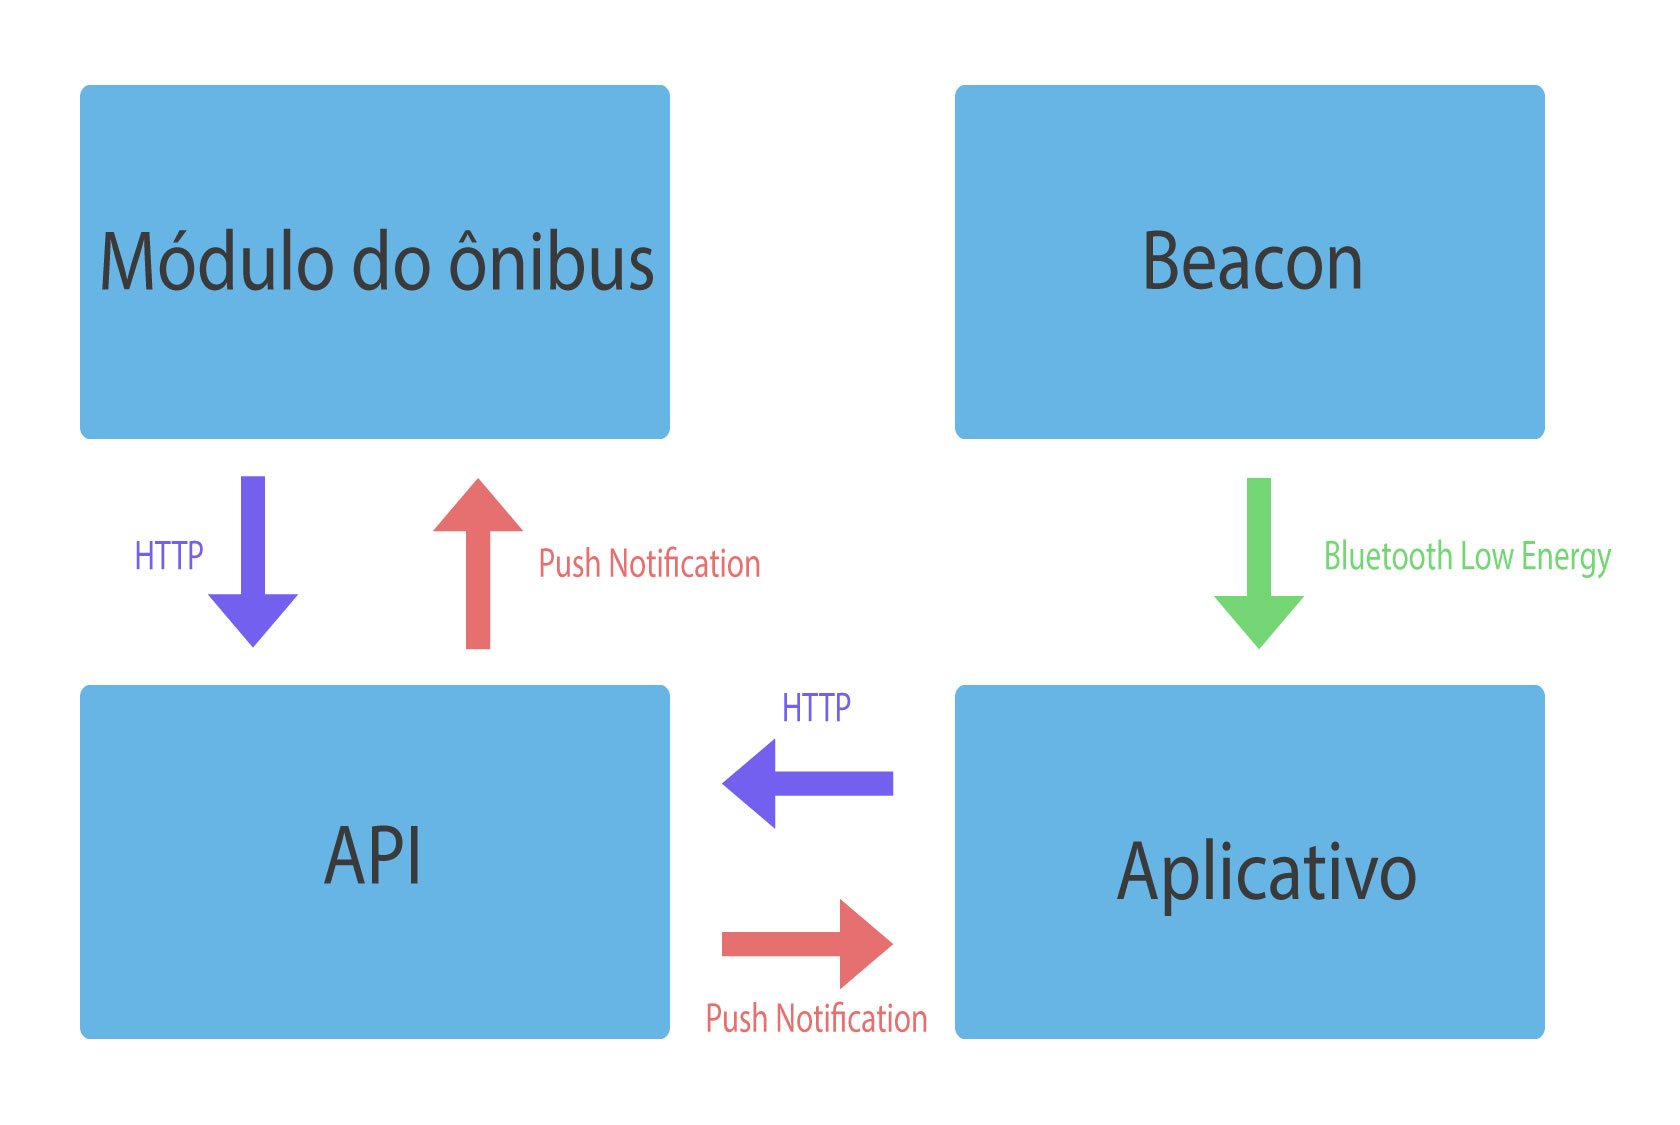
\includegraphics[width=10cm, center]{images/diagram_protocols}
\caption{Protocolos de comunicação utilizados.}
\label{Rotulo}
\end{figure}

\section{HTTP}

\textit{Hypertext Transfer Protocol} é um protocolo baseado em requisições. Quando um cliente necessita de uma informação, ele solicita para o servidor que retorna uma resposta. Sua especificação permite requisições do tipo \textit{GET, POST, DELETE}, dentre outros. Sua principal vantagem é não haver uma conexão aberta a todo momento para trafegar mensagens, permitindo que conexões e informações trafeguem apenas quando necessário. O formato para trafego das informações neste trabalho, por meio deste protocolo é a notação \textit{JSON}.

Para o cenário deste projeto, tanto o aplicativo quanto o módulo do ônibus estão em cenários não favoráveis para o trafego de informação em grande escala, tendo em vista a baixa qualidade das redes 3G/4G dos smartphones e das redes WiFi que possuem nos ônibus.

\section{Push Notification}

\textit{Push Notification} é um serviço de entrega de mensagens, parecido com \textit{SMS} (\textit{Shot Message Service}), mas que usa exclusivamente a internet para entregar. Cada plataforma possui seu próprio serviço \textit{Push}. Um bom uso deste serviço, é quando o emissor precisa enviar algo para o destinatário, sem a necessidade do destinatário ter solicitado antes, como ocorre no \textit{HTTP}.

Neste projeto temos duas situações que a tecnologia é conveniente: primeiro, existe a necessidade de avisar o motorista que é necessário, em um dado momento, parar no próximo ponto para um deficiente visual. Segundo, precisamos avisar ao deficiente visual que seu ônibus já chegou e ele pode se dirigir a ele.

Nestes dois cenários precisamos avisar os dispositivos sobre algum evento e não temos uma conexão aberta constantemente como eles. Fazendo o serviço de \textit{Push Notification} ser a melhor escolha.

Uma alternativa ao uso deste serviço são plataforma de \textit{Realtime Database}. Eles funcionam de forma parecida com o protocolo \textit{MQTT}, quando há alguma alteração em algum nó, os \textit{subscribers} são notificados sobre o novo dado.

\section{Bluetooth Low Energy}

O \textit{Bluetooth} é uma tecnologia de transmissão dados. Na sua versão 4.0+ ele se tornou \textit{BLE} (ou \textit{Bluetooth Smart}), trazendo a transmissão de dados com baixo consumo de energia.

Os pontos de ônibus não costumam possuir energia elétrica, com isso, surge a necessidade de uma tecnologia que tenha um moderado consumo de eletricidade. Com a necessidade do baixo consumo de energia e o envio constante, o \textit{BLE} em seu modo \textit{Beacons} ativado, se demonstrou ser a melhor alternativa suprindo todas as necessidades do projeto.

\chapter*{Módulo do Ponto de Ônibus}

\section{Hardware}

\begin{enumerate}
\item HM-10 - Bluetooth 4.0 BLE module
\item Arduino Uno
\end{enumerate}

Arduino Uno é utilizado apenas como ponte para configurar o módulo HM-10. A ligação deve seguir o diagrama abaixo.


\begin{figure}[!h]
\centering
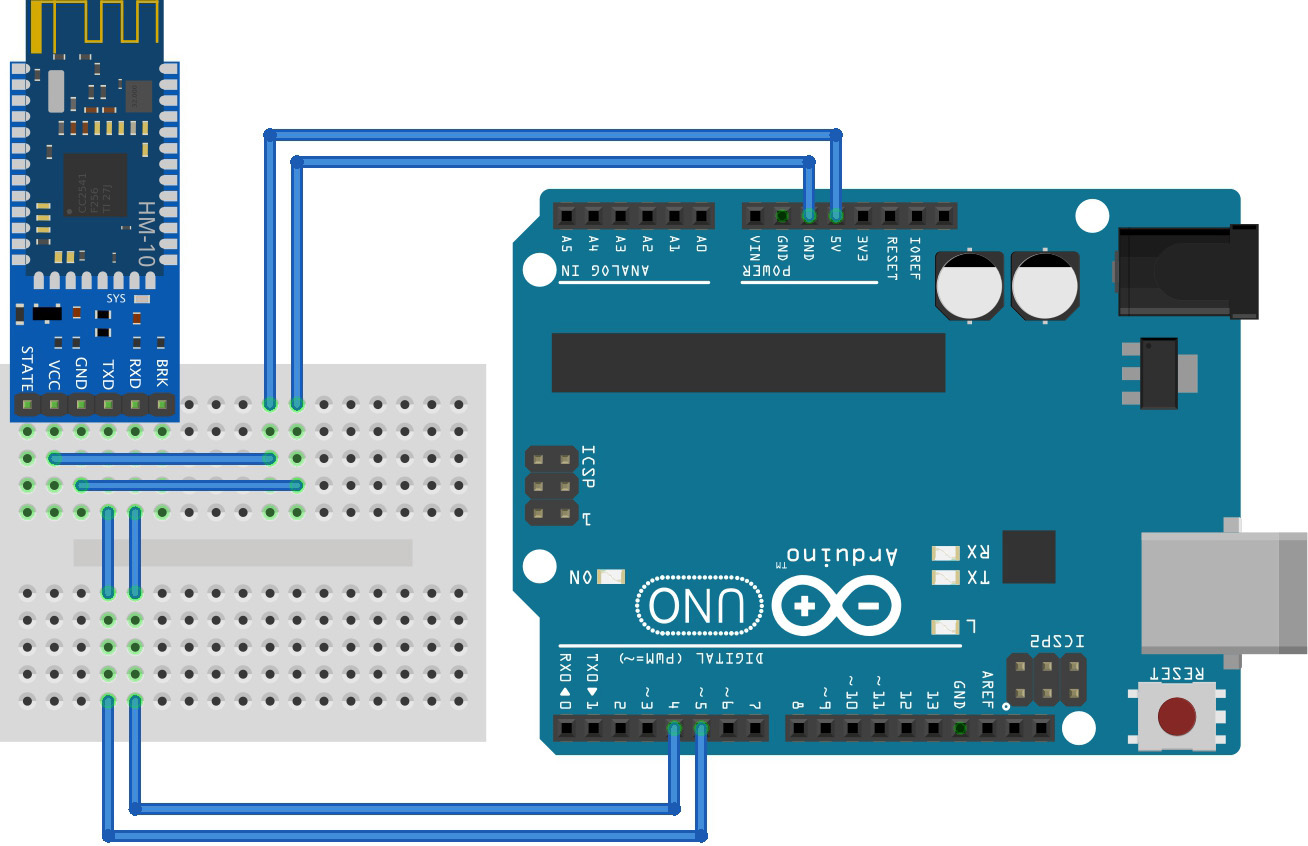
\includegraphics[width=10cm, center]{images/arduino-hm10}
\caption{Módulo Bluetooth HM10.}
\label{Rotulo}
\end{figure}

\section{Software}

\begin{itemize}
\item Arduino IDE 1.8.3 ou superior. 
\end{itemize}

\section{Configuração}

Conecte o arduino Uno ao computador e compile o código abaixo utilizando a IDE do arduino.

\lstinputlisting[style=customc]{codes/arduino-code.ino}

Após compilador, utilizando o Serial Monitor da IDE, execute os comandos AT na seguinte ordem:

Obs: Quanto menor o tempo de envio, maior a economia de energia.

\begin{enumerate}
\item AT+RENEW //Coloca nos padrões de fábrica
\item AT+RESET //Reinicia para aplicar os padrões de fábrica
\item AT+MARJ0xNNNN //Define o valor Marjor
\item AT+MINO0xNNNN //Define o valor Minor
\item AT+NAMEMeuBeacon //Define o nome do Beacon
\item AT+ADVI5 //Define tempo de envio. 5 = 546.25 millisegundos
\item AT+ADTY3 //Define como não pareável
\item AT+IBEA1 //Habilita como Beacon
\item AT+DELO2 //Configura para apenas emitir sinal
\item AT+PWRM0 //Habilita auto-sleep para economizar energia
\item AT+RESET
\end{enumerate}


Após configurado, pode ser ligado em uma bateria 3v para utilização.

\section{Referências}

\href{ftp://imall.iteadstudio.com/Modules/IM130614001_Serial_Port_BLE_Module_Master_Slave_HM-10/DS_IM130614001_Serial_Port_BLE_Module_Master_Slave_HM-10.pdf}{HM-10 Bluetooth 4.0 BLE module Datasheet}
\\
\href{https://www.arduino.cc/en/main/software}{Arduino IDE}
\\
\href{https://github.com/metractive/beacon-study}{Repositório da Metractive - Como construir Beacons}

\chapter*{Módulo do Ônibus}

\section{Hardware}

\begin{itemize}
\item Intel Edison
\item Raspberry Pi 3
\item Tela LCD 7" (em breve)
\item NEO u-blox 6 GPS Modules
\end{itemize}

\subsection{Intel Edison}

\begin{figure}[!h]
\centering
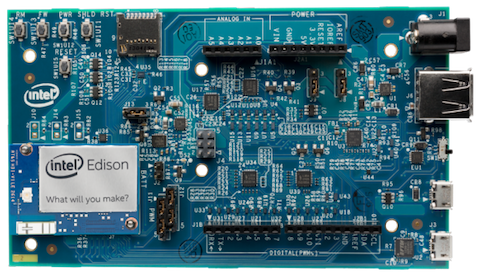
\includegraphics[width=10cm, center]{images/intel-edison-arduino-kit}
\caption{Intel Edison.}
\label{Rotulo}
\end{figure}

Inicialmente foi adotado o Intel Edison com placa de expansão arduino. Foi escolhido devido a fácil acesso a um exemplar e ótimo hardware. Ele conta com WiFi, Bluetooth, portas I/O, processador Intel Atom de 500 MHz, 1GB de memória RAM DDR3 e 4GB eMMC. \\
Sua utilização foi fácil e não obtivemos nenhuma dificuldade em instalar o sistema que escolhemos.


Problemas encontrados em adotar como solução:
\\

\textbf{Preço}

Embora tenha um ótimo hardware e uma empresa séria por trás da sua construção, o preço, em 07/2017, que gira em torno de R\$ 600,00, não justifica sua adoção como a melhor solução para o projeto já que existem alternativas com preços melhores e bom desempenho.
\\

\textbf{Ausência de controlador gráfico}

Uma das features do projeto é emitir alertas visuais para o motorista por meio de telas LCDs. A placa Intel Edison nos permite fazer alertas visuais utilizando LEDs e afins. 
\\

\textbf{Descontinuidade da placa pela Intel}

em 07/2017, a Intel anunciou a descontinuidade do desenvolvimento de algumas placas que fabrica. O Intel Edison foi uma delas.

\subsection{Raspberry Pi 3}

\begin{figure}[!h]
\centering
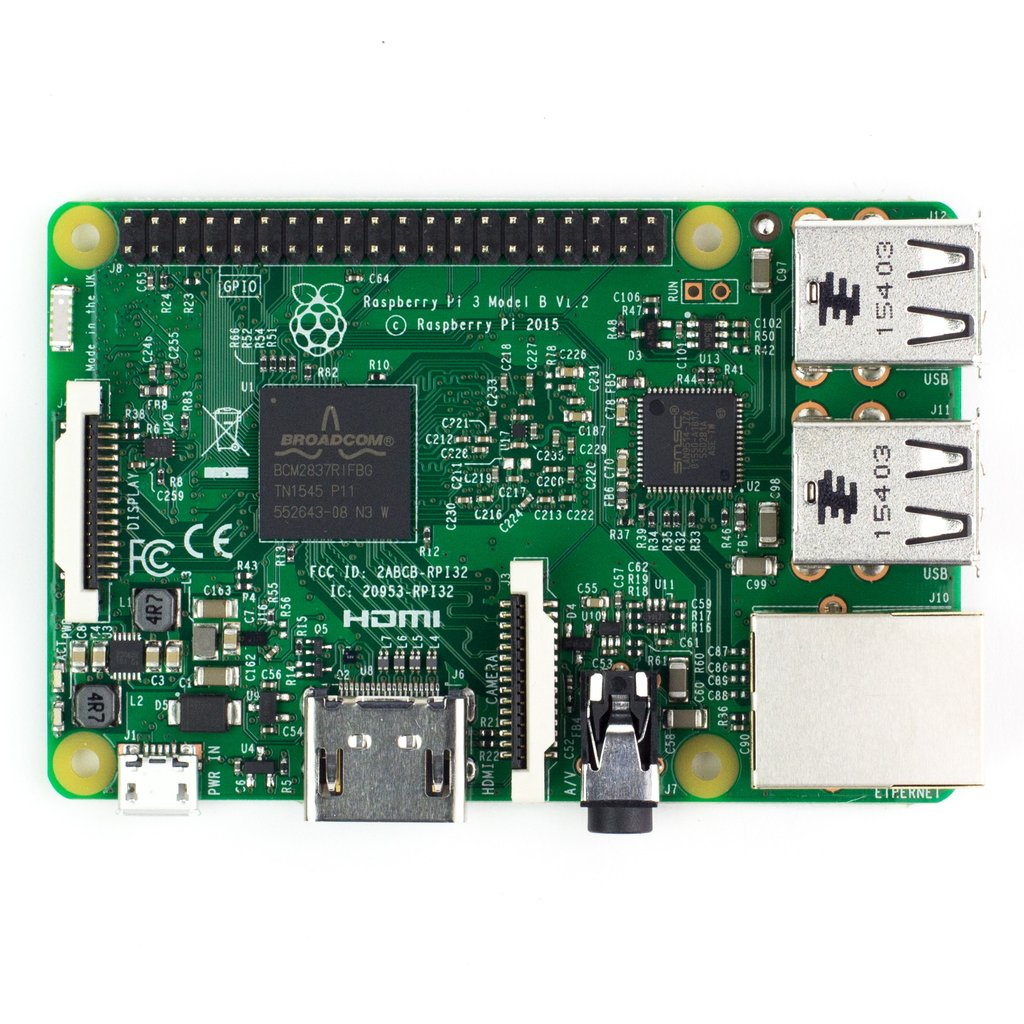
\includegraphics[width=10cm, center]{images/raspberry-pi}
\caption{Raspberry 3.}
\label{Rotulo}
\end{figure}

Testes realizados no Raspberry Pi 3 demonstraram ser uma boa alternativa ao Intel Edison. Foi fácil a instalação do sistema e a placa vem com saída HDMI permitindo utilizar telas LCD para fazer os alertas visuais.
Seu preço, em 08/2017, gira em torno de R\$ 150,00, 1/4 do preço do Intel Edison. Seu hardware contém boas especificações:

\begin{itemize}
\item Quad Core 1.2GHz Broadcom BCM2837 64bit CPU
\item 1GB RAM
\item BCM43438 wireless LAN and Bluetooth Low Energy (BLE) on board
\item 40-pin extended GPIO
\item 4 USB 2 ports
\item 4 Pole stereo output and composite video port
\item Full size HDMI
\item CSI camera port for connecting a Raspberry Pi camera
\item DSI display port for connecting a Raspberry Pi touchscreen display
\item Micro SD port for loading your operating system and storing data
\item Upgraded switched Micro USB power source up to 2.5A
\end{itemize}

Embora tenha um hardware com especificações superiores ao Intel Edison, não houve ganho de desempenho ao rodar o sistema, devido a ausência de algoritmos complexos no sistema. Assim, a grande vantagem de se utilizar o Raspberry Pi 3 ao invés do Intel Edison, é seu baixo custo e recurso de chip gráfico.

\subsection{Módulo NEO u-blox 6 GPS}

\begin{figure}[!h]
\centering
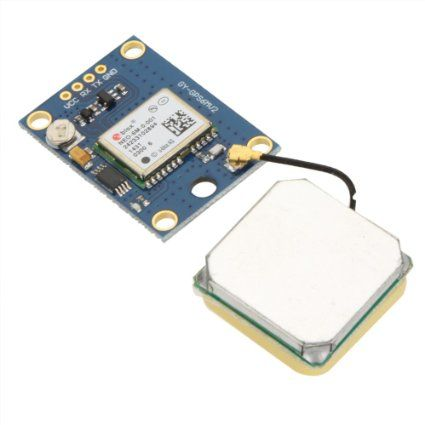
\includegraphics[width=10cm, center]{images/neo-6m}
\caption{Módulo NEO u-blox 6 GPS.}
\label{Rotulo}
\end{figure}

Para realizar o rastreamento do ônibus foi adotado o módulo NEO u-blox 6 GPS Modules, devido a compatibilidade com as placas que contém o sistema embarcado e preço acessível. 

\textbf{Localização}

Uma característica desse módulo é trabalhar com GPS, fazendo comunicação direta com no mínimo 3 satélites para triangular sua posição com mais precisão. Alguns módulos disponíveis no mercado trabalham com A-GPS, que usam torres de telefonia móvel para conhecer sua posição.
O uso do GPS trás maior precisão, porém demora mais para estabelecer conexão com satélites. O A-GPS fornece a localização com menor tempo, porém com menor precisão e a um custo mais alto.

\textbf{Comunicação}

O módulo realiza comunicação UART (Universal Asynchronous Receiver/Transmitter), o que permite fácil comunicação com as placas utilizadas para testes.

\textbf{Preço}

Seu preço, em 08/2017, gira em torno de R\$ 60,00 e pode ser encontrado com facilidade na internet para venda. 


\section{Software}

\subsection{Sistema Operacional}

\textbf{Android Things}
Em 2016 o Google anunciou o Android Things, uma versão do Android voltada para IoT (Internet of Things). Ele é, atualmente, uma versão do Android Marshmallow reduzida. Sua escolha foi devido a facilidade de embarcar em placas como o Raspberry Pi e Intel Edison, e a variedade de recursos que já estão disponíveis no SO que facilitam o desenvolvimento do módulo, como o recurso LocationManager. \textbf{[Detalhar mais essa parte]}

\subsection{IDE}

Foi escolhido o Android Studio como IDE do projeto. Ela é desenvolvida pela IntelliJ e tida pelo Google como ferramenta oficial de desenvolvimento para aplicativos Android.

\subsection{Linguagem}

O Google tem duas linguagens de primeiro nível para desenvolvimento Android: Java e Kotlin. Para esse projeto adotamos a linguagem Kotlin, que possui sintaxe muito simplificado em comparação ao Java. Embora Java tenha sido a primeira linguagem oficial para desenvolvimento, Kotlin oferece acesso aos mesmo recursos do sistema.
Algumas bibliotecas disponíveis, desenvolvidas por terceiros, ainda não migraram para o Kotlin, obrigando a implementar algumas classes em Java. Como Kotlin tem interoperabilidade com Java, não existe nenhum impeditivo de utilizar Kotlin e eventualmente alguma classa Java.

\subsection{Arquitetura}

\begin{figure}[!h]
\centering
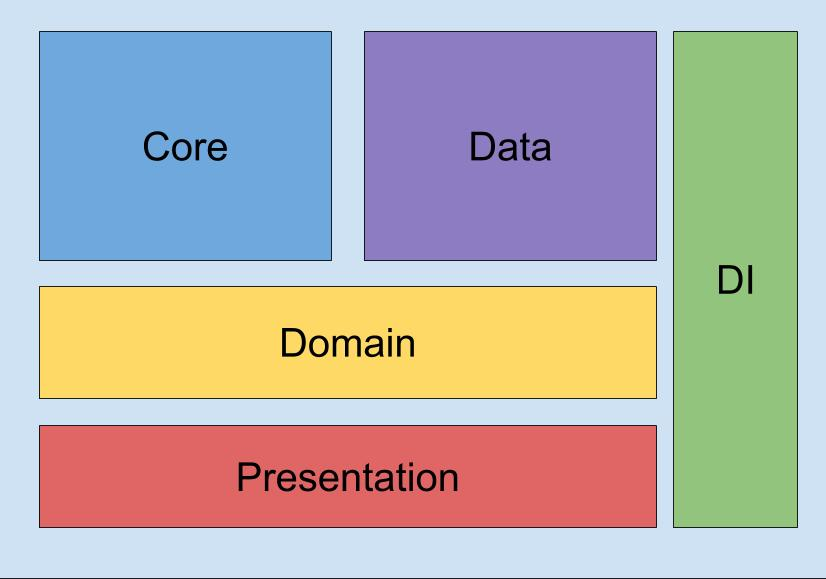
\includegraphics[width=10cm, center]{images/brick_diagram_bus_tracker}
\caption{Diagrama de bloco do módulo do ônibus.}
\label{Rotulo}
\end{figure}

Para desenvolvimento do software, foi adotado o padrão \textit{Clean Archtecture}. É um padrão que visa um maior desacoplamento das classes e distruibui bem as responsabilidades.

\begin{description}

\item[Core] Não contém nenhuma lógica de negócio. Esta camada provê informações comuns, como configurações estáticas da placa a toda a aplicação. Possui também algumas classes e interfaces bases.

\item[Data] Responsável por prover dados para toda aplicação. Ela adota o Padrão de Arquitetura \textit{Repository}, tendo uma interface de acesso aos dados. Uma grande vantagem em utilizar essa camada com esse padrão de arquitetura, é o respeito a responsabilidade única, um dos princípios do \textit{SOLID}. Ela encapsula toda lógica de busca de dados, assim, caso uma classe precise de algum dado específico, ela solicita através da interface de comunicação e a classe que implementa a interface, cuida de toda lógica de busca de dado, seja um dado armazenado localmente, em cache ou em um servidor remoto. Tudo fica transparente para a classe que solicitou o dado.

\item[Domain] Esta camada encapsula toda regra de negócios da aplicação. Toda vez que é necessário realizar processamentos em dados para satisfazer funcionalidades, é feito por esta camada.

\item[Presentation] Responsável por toda interface gráfica. Toda lógica de criação de telas e interceptação de interações do usuário com o aplicativo, é feito aqui. Quando é necessário procurar dados para exibir ao usuário, é feito solicitações deles para a camada Domain ou Data para que seja possa exibir os dados.
 
\end{description}

\section{Referências}

%links do intel edison
\href{https://software.intel.com/en-us/iot/hardware/edison}{Site Oficial Intel Edison}\\
\href{http://download.intel.com/support/edison/sb/edisonmodule_hg_331189004.pdf}{Datasheet Intel Edison}\\
\href{https://www.embarcados.com.br/placas-intel-edison-galileo-e-joule-serao-descontinuadas/}{Anúncio do fim da produção do Intel Edison}\\
%links do raspberry pi
\href{https://www.raspberrypi.org/products/raspberry-pi-3-model-b/}{Site Oficial Raspberry Pi}\\
\href{https://www.raspberrypi.org/documentation/hardware/computemodule/RPI-CM-DATASHEET-V1_0.pdf}{Datasheet Raspberry Pi 3}\\
%links do módulo GPS
\href{https://www.u-blox.com/sites/default/files/products/documents/NEO-6_DataSheet_(GPS.G6-HW-09005).pdf}{Datasheet NEO u-blox 6 GPS Modules}\\
%android things
\href{https://developer.android.com/things/index.html}{Site Oficial Android Things}\\
\href{https://developer.android.com/things/hardware/edison.html}{Configuração do Android Things no Intel Edison}\\
\href{https://developer.android.com/things/hardware/raspberrypi.html}{Configuração do Android Things no Raspberry Pi 3}\\

\chapter*{Aplicativo}

\section{Telas}


\begin{figure}[!h]
\centering
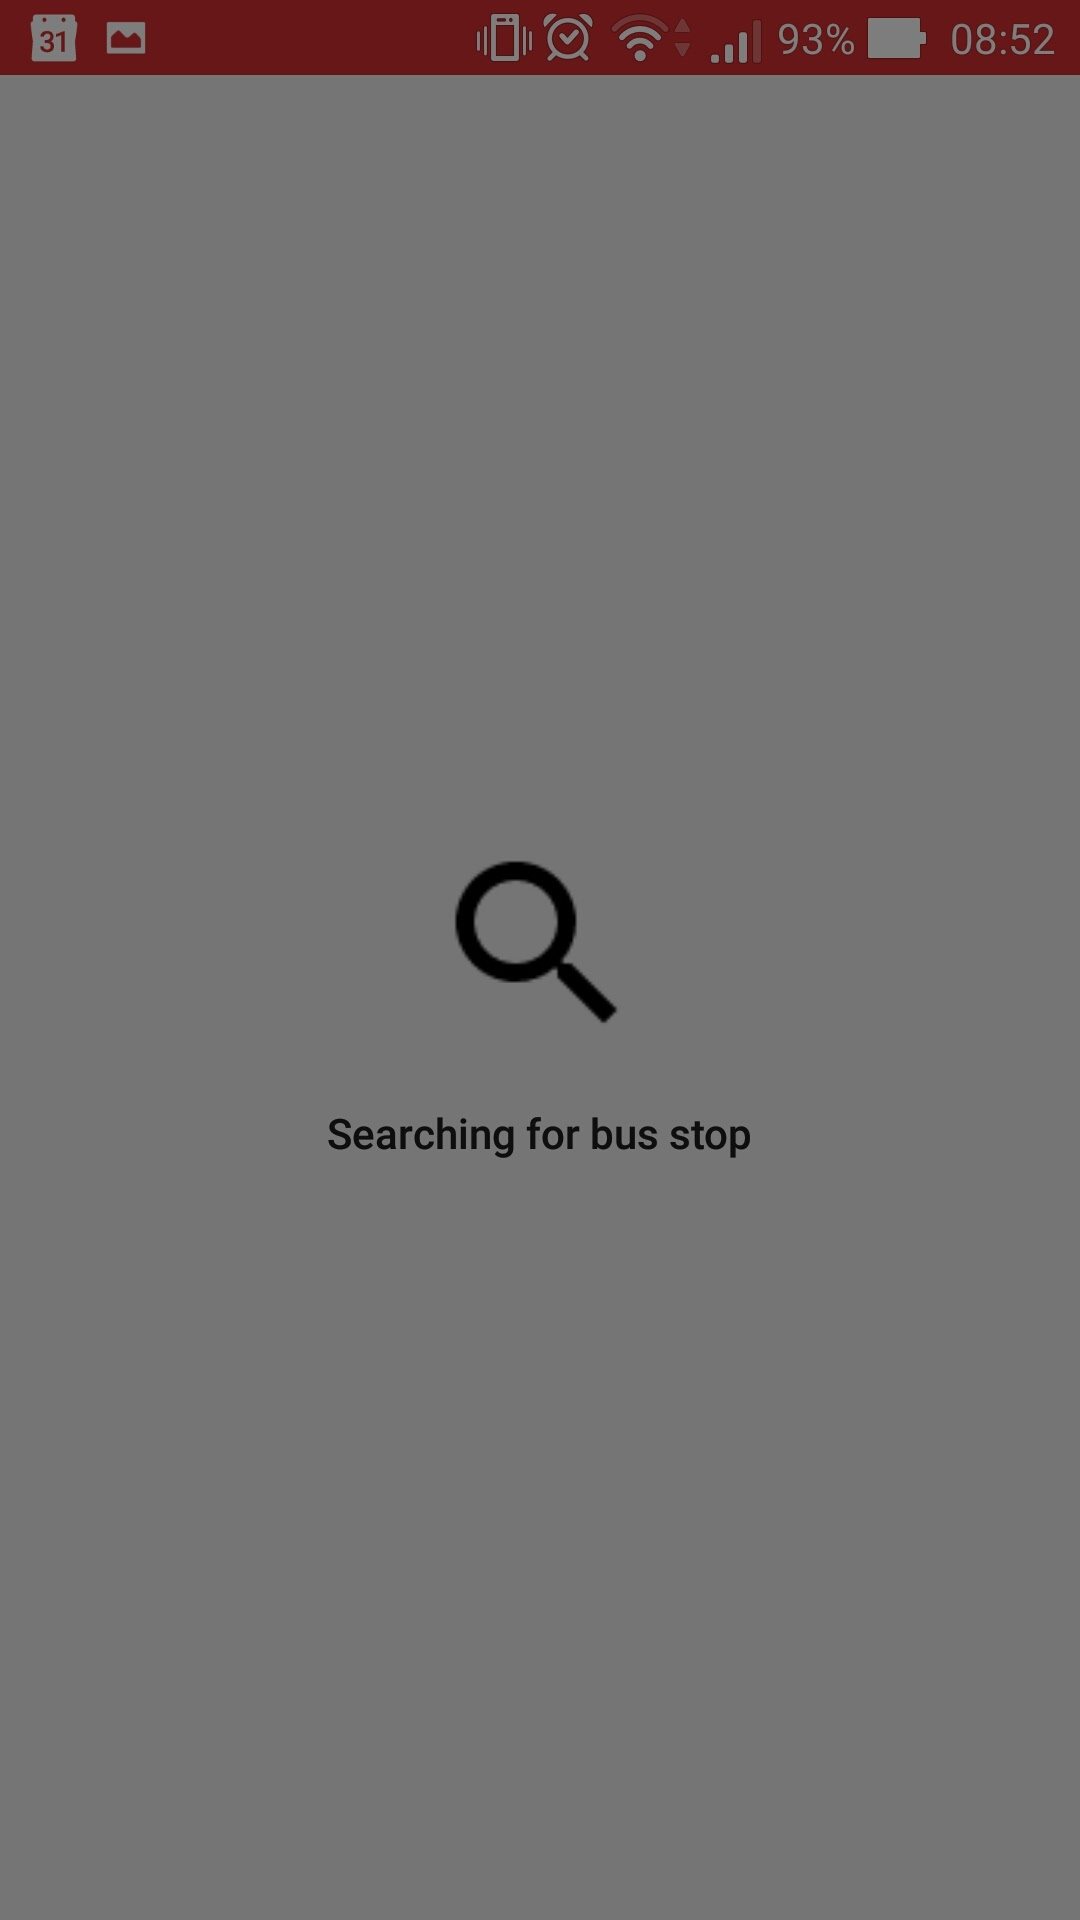
\includegraphics[width=5cm, center]{images/beacon_searching_bus_stop}
\caption{Tela de busca por um ponto de ônibus do aplicativo móvel.}
\label{Rotulo}
\end{figure}

\begin{figure}[!h]
\centering
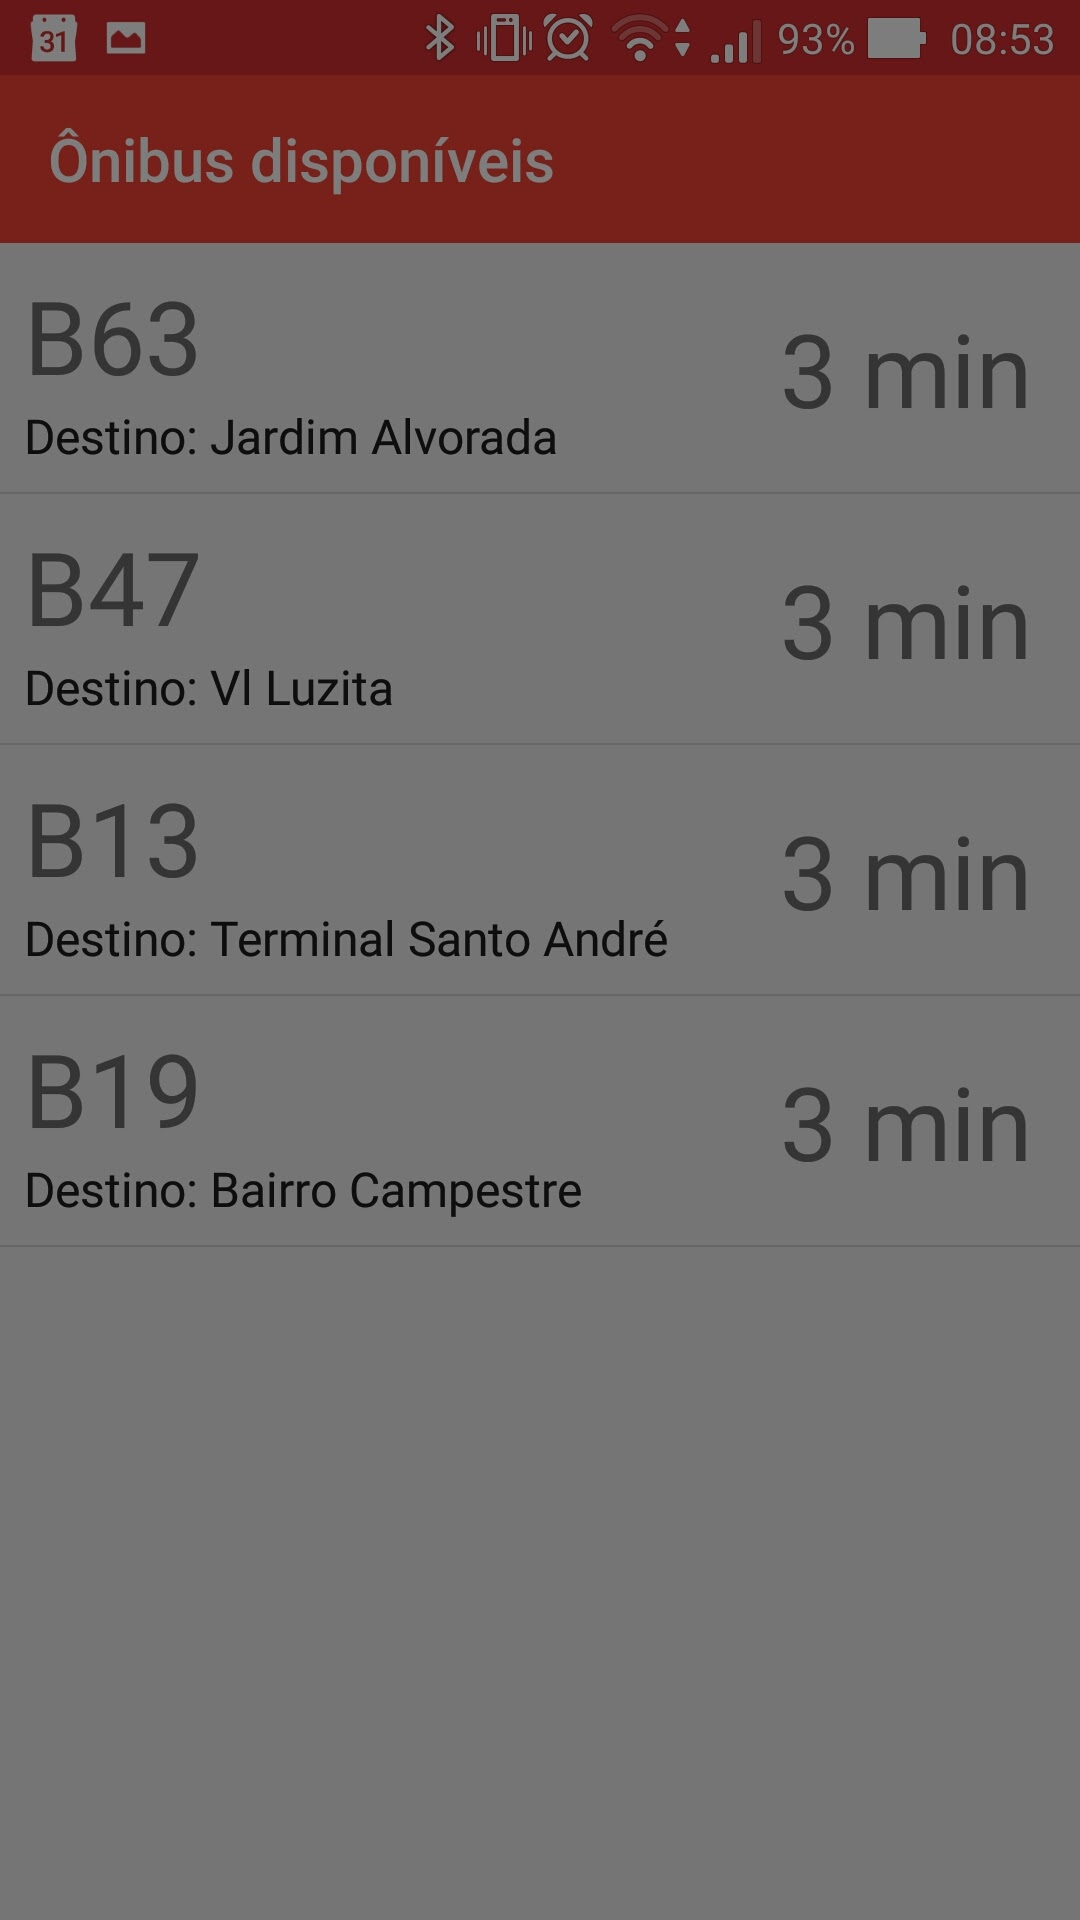
\includegraphics[width=5cm, center]{images/beacon_list_bus}
\caption{Tela com lista de ônibus disponíveis do aplicativo móvel.}
\label{Rotulo}
\end{figure}

\begin{figure}[!h]
\centering
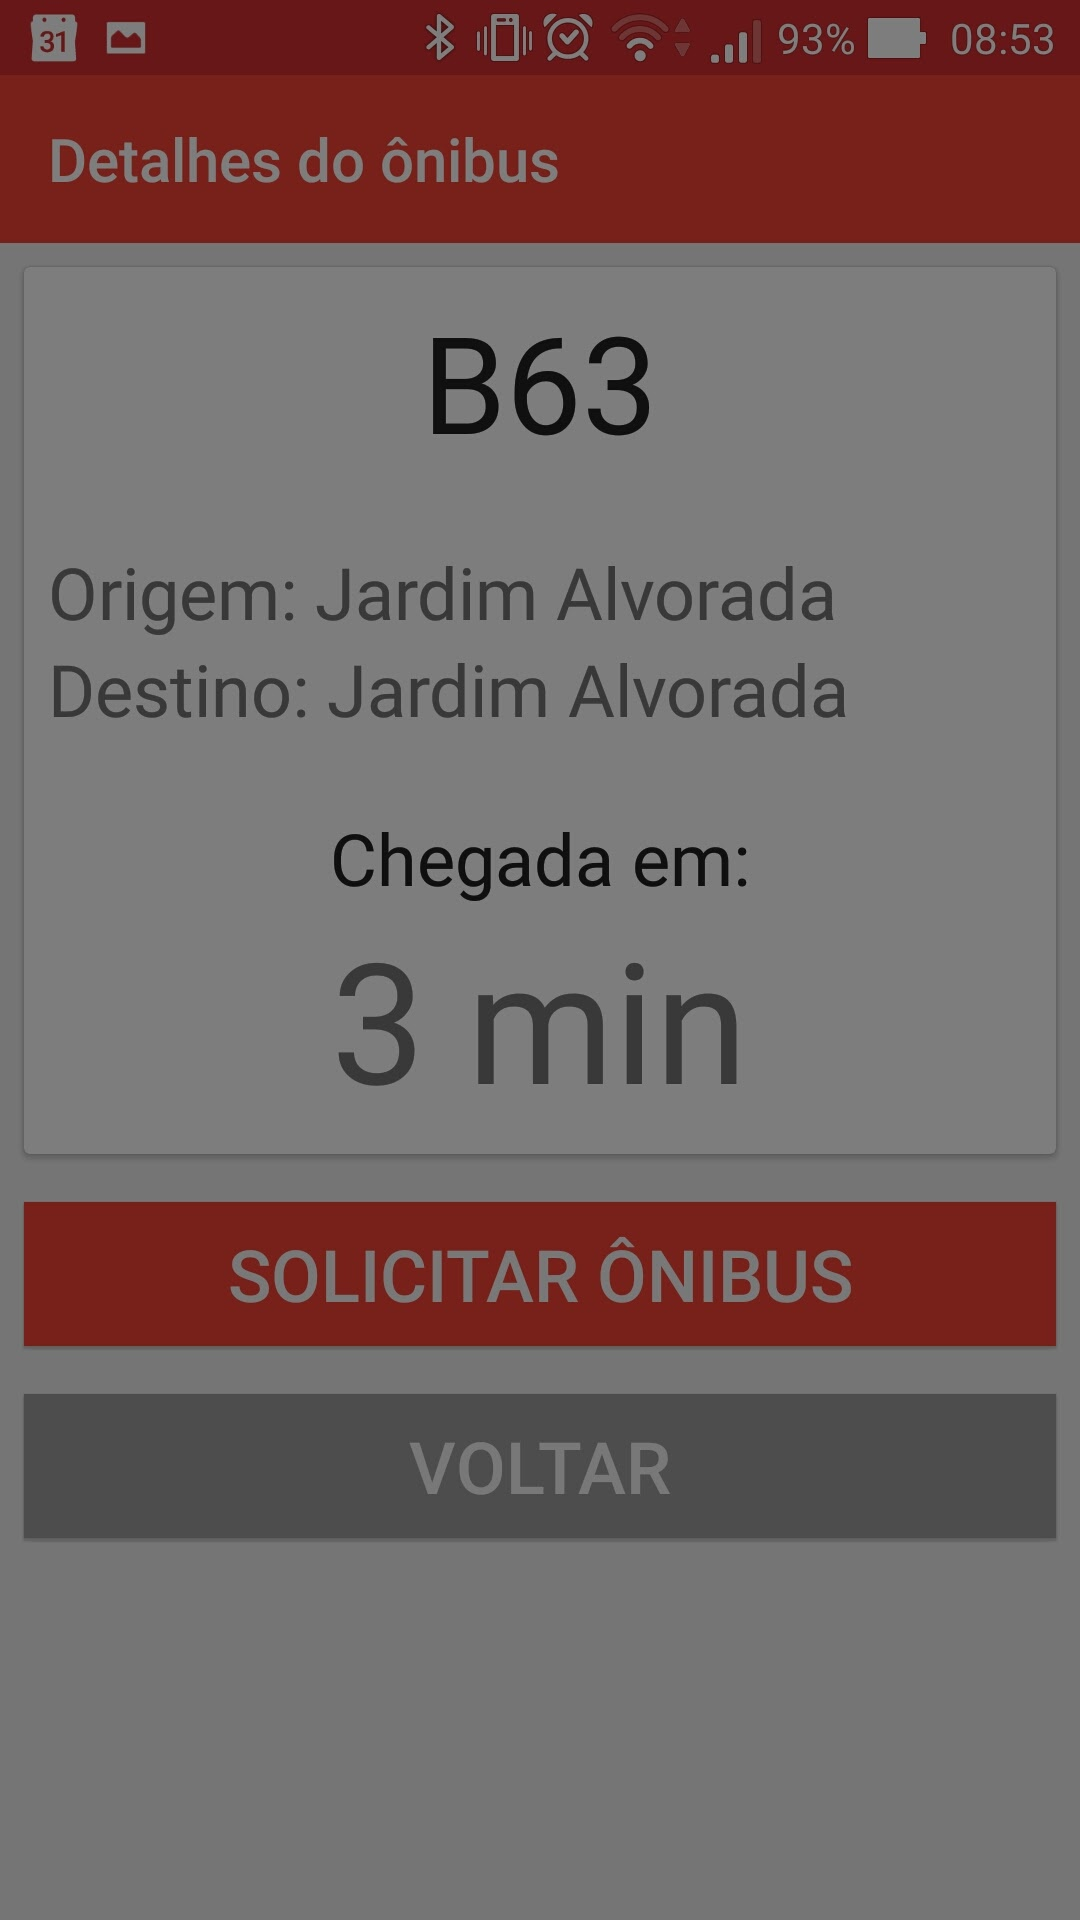
\includegraphics[width=5cm, center]{images/beacon_detail_bus}
\caption{Tela com detalhes do ônibus do aplicativo móvel.}
\label{Rotulo}
\end{figure}

\section{IDE}

Foi escolhido o Android Studio como IDE do projeto. Ela é desenvolvida pela IntelliJ e tida pelo Google como ferramenta oficial de desenvolvimento para aplicativos Android.

\section{Linguagem}

O Google tem duas linguagens de primeiro nível para desenvolvimento Android: Java e Kotlin. Para esse projeto adotamos a linguagem Kotlin, que possui sintaxe muito simplificado em comparação ao Java. Embora Java tenha sido a primeira linguagem oficial para desenvolvimento, Kotlin oferece acesso aos mesmo recursos do sistema.
Algumas bibliotecas disponíveis, desenvolvidas por terceiros, ainda não migraram para o Kotlin, obrigando a implementar algumas classes em Java. Como Kotlin tem interoperabilidade com Java, não existe nenhum impeditivo de utilizar Kotlin e eventualmente alguma classa Java.

\section{Arquitetura}

\begin{figure}[!h]
\centering
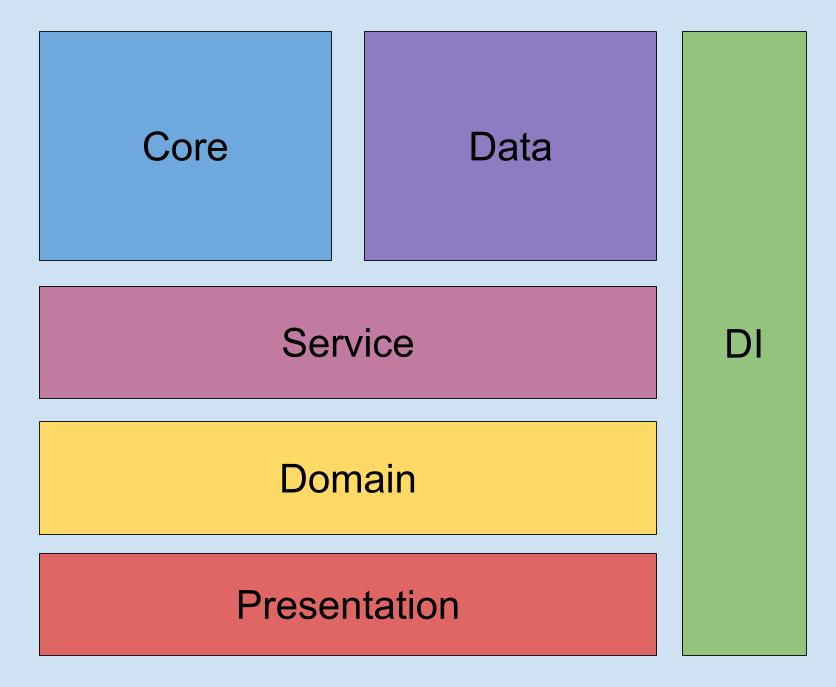
\includegraphics[width=10cm, center]{images/brick_diagram_beacon}
\caption{Diagrama de blocos do aplicativo móvel.}
\label{Rotulo}
\end{figure}

Para desenvolvimento do software, foi adotado o padrão \textit{Clean Architecture}. É um padrão que visa um maior desacoplamento das classes e distruibui bem as responsabilidades.

\begin{description}

\item[Core] Não contém nenhuma lógica de negócio. Esta camada provê informações comuns, como configurações estáticas da placa a toda a aplicação. Possui também algumas classes e interfaces bases.

\item[Data] Responsável por prover dados para toda aplicação. Ela adota o Padrão de Arquitetura \textit{Repository}, tendo uma interface de acesso aos dados. Uma grande vantagem em utilizar essa camada com esse padrão de arquitetura, é o respeito a responsabilidade única, um dos princípios do \textit{SOLID}. Ela encapsula toda lógica de busca de dados, assim, caso uma classe precise de algum dado específico, ela solicita através da interface de comunicação e a classe que implementa a interface, cuida de toda lógica de busca de dado, seja um dado armazenado localmente, em cache ou em um servidor remoto. Tudo fica transparente para a classe que solicitou o dado.

\item[Service] Provê serviços para qualquer camada. No caso do aplicativo, a implementação do serviço de voz fica neste pacote e é injeta pelo pacote de Injeção de Dependências.

\item[Domain] Esta camada encapsula toda regra de negócios da aplicação. Toda vez que é necessário realizar processamentos em dados para satisfazer funcionalidades, é feito por esta camada.

\item[Presentation] Responsável por toda interface gráfica. Toda lógica de criação de telas e interceptação de interações do usuário com o aplicativo, é feito aqui. Quando é necessário procurar dados para exibir ao usuário, é feito solicitações deles para a camada Domain ou Data para que seja possa exibir os dados.

\item[DI] Este projeto utiliza o padrão de arquitetura \textit{Injeção de Dependências}. Esta camada provê todas dependências, fazendo a implementação mais limpas nas outras classes, já que não precisam saber como instânciar uma classe, apenas usam.
 
\end{description}

\section{Áudio Descrição}

Uma das funcionalidades do aplicativo é descrição da tela que o deficiente está. O \textit{TalkBack} fala para o usuário em qual componente ele está tocando, porém, não descreve em qual tela ele acabou de entrar. 
A implementação por áudio descrição foi simples com uso da API nativa \textit{TextToSpeech}, onde podemos passar textos personalizados e o serviço se encarrega de sintetizar a voz.

O uso de uma camada de DI (Injeção de Dependências) facilitou o processo de implementação, fazendo ela na camada de serviço e configurando a instanciação no padrão \textit{Singleton} para que todos que vão utilizar (nesse caso são os \textit{presenters}), apenas solicitem a instância sendo passada por construtor.

\chapter*{Web service}

\section{Linguagem}

Para o desenvolvimento do \textit{web service} foi escolhida a utilização da pilha MEAN, que engloba quatro tecnologias para desenvolvimento \textit{web} que possuem como base a linguagem JavaScript.


\subsection{JavaScript}

JavaScript é uma linguagem de programação \textit{client-side}, utilizada para manipular os comportamentos de uma página, controlando o HTML e o CSS. Outra característica dela, é que ela é uma linguagem orientada à eventos.
Para explicar melhor o que são eventos, é importante citar que uma página HTML utiliza tags para representar seus elementos, podendo conter menus, botões e formulários em seu corpo. Cada elemento possui alguns atributos, sendo alguns desses atributos de eventos, como por exemplo o \textit{onClick} que realiza alguma função caso o elemento referente seja clicado pelo usuário.
Tais funções podem ser desenvolvidas em JavaScript, entrando aqui para dizer qual comportamento a página terá ao disparo do evento.\\

\section{MEAN stack}

A pilha \textit{MEAN} é um conjunto de \textit{frameworks} desenvolvidos em JavaScript, que englobam os lados do cliente, do servidor e do banco de dados. Por possuírem a mesma linguagem como base, os elementos dessa pilha contam com uma maior produtividade no desenvolvimento. MEAN é um acrônimo para MongoDB, Express, Angular e Node.


\subsection{MongoDB}

É um banco de dados não relacional com uma escalabilidade muito boa. Ele utiliza conceitos de \textit{collections} e \textit{documents} em sua construção. 
As \textit{collections} são equivalentes aos bancos de um ambiente que utiliza o SQL. Já os \textit{documents}, se equivalem aos registros de cada banco.
Os dados são guardados em arquivos similares aos de formato JSON (\textit{JavaScript Object Notation}).
Outro item importante sobre o MongoDB é o fato de ser schemaless, tornando-o bem flexível em relação a inclusão de dados diferentes em uma mesma \textit{collection}, fazendo com que a validação de dados fique nas mãos dos desenvolvedores.


\subsection{Express}

É um framework que ajuda na organização de sua aplicação, caso use a arquitetura MVC, no lado do servidor. Uma de suas funções é a de facilitar a criação e manutenção de rotas, realizando uma configuração inicial com os caminhos para os \textit{controllers, models} e \textit{views} utilizados pela sua aplicação, além de informar os dados de configuração do servidor.


\subsection{Angular}

Framework utilizado no lado do cliente. Possui um conjunto adicional de atributos para as páginas HTML, passando parte do processamento dos dados da página para o lado do cliente. Isso possibilita a criação de interfaces dinâmicas e assíncronas além de diminuir a carga de processamento do servidor.


\subsection{Node}

Plataforma principal para o funcionamento da pilha MEAN. Ele utiliza o gerenciador de pacotes npm para organizar as bibliotecas utilizadas pela sua aplicação. É ele que realiza a conexão com servidores e diz quais bancos de dados serão utilizados pela aplicação.


\section{Dificuldades}

Apesar de conter conceitos simples de aprender, devido à grande quantidade de métodos para se realizar os mesmos processos, fica um pouco difícil para assimilar quais os arquivos que devem ser modificados para o funcionamento adequado da aplicação.
Primeira dificuldade surgiu ao utilizar o mongoose, uma solução baseada em \textit{schemas} para o banco de dados MongoDB que cuida de validações e tipagem de dados, resolvido ao criar arquivos separados para cada \textit{collection} do banco.


\section{Referências}

%links do HTML
\href{https://www.w3schools.com/tags/ref_eventattributes.asp}{Atributos de eventos}\\
%links do javascript
\href{http://tableless.github.io/iniciantes/manual/js/}{Guia introdutório sobre JavaScript}\\

%links do MEAN stack
ALMEIDA, Flávio. MEAN - Full stack JavaScript para aplicações web com MongoDB, Express, Angular e Node. ed. Casa do Código, 2016.\\
%links do push notifications

Falar sobre o MEAN stack e sobre as dificuldades que estou encontrando sobre como trabalhar com cada tecnologia da pilha.

\end{document}